\documentclass[glenn,refnum,codigo]{Estilo}
%%%
\usepackage[most]{tcolorbox}
\tcbset{colframe=estilo!90!black,colback=estilo!15,fonttitle=\bfseries\sffamily}
%%%
%%% Para a identificação da monografia
%%%
\title{Zero, o nada que existe}
\autor{Benaia Sobreira de Jesus Lima}
%%%
%%% Banca Examinadora
%%%
\orientador[m]{Susan Wouters}
\segundo{Prof. Dr. Marcello Fidelis}
\terceiro{Prof. Dr. Aleksandro de Mello}
\grandedia{\today} %%% Substitua \today pelo dia da defesa de sua monografia
\matricula{96190051}
\controle{$1$} %%% A classe estilo completa com o ano, relaxe.
\grauL{Licenciado}
%%%
%%%
\begin{document}
%%%
%%%
\frontmatter %%% Necessário para os ajustes da parte pre-textual
%%%
\capa  %%% Esse comando cria a capa
%%%
\rosto %%% Esse comando cria a folha de rosto
%%%
\epigrafe{A vida gosta de quem gosta dela.}{Alguém}

\begin{dedico}
	A dedicatória é opcional, caso queira dedicar seu trabalho a alguém, ponha sua dedicatória aqui.
\end{dedico}

\begin{agradece}
	Os agradecimentos também são opcionais, mas é sempre bom fazer. Ponha aqui seus agradecimentos.
\end{agradece}

\begin{resumo}
	
	O resumo é obrigatório, insira o seu aqui
	
	\palavras{Zero, número, história}.
\end{resumo}

\begin{resumoE}
	
	Your resumo in English.
	
	\palavrasE{Zero, number, history}.
\end{resumoE}

\tableofcontents    %%% Sumário
%%%\listoffigures   %%% Lista de figuras
%%%\listoftables    %%% Lista de tabelas
%%%
\introducao

Os números naturais tiveram suas origens nas necessidades de contagem.
Esse é o motivo histórico (existem outros) pelo qual zero não é considerado
número natural por muitos, pois a contagem sempre começa com o número um.

Os primeiros passos para a abstração vieram com o uso de numerais para
representar números. A partir daí surgiram sistemas para representação
de grandes números. Por exemplo, os babilônicos construíram um eficiente
sistema de atribuição de valor baseado nos numerais de $1$ a $10$. Os
egípcios possuíam um sistema com símbolos (hieróglifos) distintos para
as potências de $10$ menores que um milhão.

Uma gravação em pedra encontrada em Karnak-Egito, datando de cerca
de $1500$ a.C. e atualmente no Louvre, em Paris, representa $276$
como $2$ centenas, $7$ dezenas e $6$ unidades, exatamente como o fazemos
hoje com nosso sofisticado sistema decimal posicional.

O avanço na abstração foi muito lento, a idéia do zero como um número
a ser usado em um sistema posicional com seu próprio numeral passou
despercebida a muitas mentes brilhantes. Os babilônicos, desde cerca
de $700\, a.C.$ usavam zero como notação de posição, porém eles nunca
o utilizaram como elemento final.

Os \textbf{Olmecas} e a civilização \textbf{Maia} utilizaram o
zero como um número separado desde o século I AC, porém seu uso não
se difundiu na Mesoamérica. O conceito, como é  utilizado atualmente,
se originou na Índia com o matemático Brahmagupta, por volta de $628$.

O primeiro estudo axiomático dos números (como entidades abstratas)
geralmente é atribuí-do aos filósofos gregos Pitágoras e Arquimedes.
No entanto, na mesma época, ocorreram estudos independentes na Índia,
China e Mesoamérica.\index{Números!Pitágoras}\index{Números!Arquimedes}

Só no final do século $XIX$, com o matemático italiano Giuseppe Peano,
o conjunto dos números naturais foi contemplado com uma definição
teórica formal, consistente e precisa. Segundo esta definição, era
conveniente que o zero (correspondente ao conjunto vazio) fosse um
número natural.


Essa convenção, em geral, é seguida por quem se interessa pela
teoria dos conjuntos, algebristas, logicistas e cientistas da
computação. Quem se interessa por análise ou teoria dos números
normalmente prefere excluir o zero dos números naturais.

A construção do conjunto dos Números Naturais dada por Giuseppe Peano
é atualmente conhecida como Axiomas de Peano, é uma estrutura simples
e elegante, que serve como exemplo didático de construção de conjuntos
numéricos.

Em $1889$ Giuseppe Peano, em seu livro ``Arithmetices
Principia Nova Methodo Exposita"  estabeleceu alguns axiomas para
a aritmética. Três deles permitem cons\-truir formalmente o conjunto
dos números Naturais, o qual denota-se por $\N$. Segue os Axiomas
(ou postulados) de Peano\index{Números Naturais!Axiomas de Peano}
\index{Axiomas de Peano!Números Naturais}.


\begin{Lista}
	\item Existe um número 0;
	\item Todo número $n$ tem um sucessor $s(n)$ no mesmo conjunto;
	\item Se $n\neq{m}$ então $s(n)\neq{s(m)}$.
\end{Lista}

O conjunto dos números Naturais $\N$ é apenas um modelo para os axiomas
de Peano em que a operação de sucessão é definida por $s(n) = n + 1$, assim
\[
\N = \{0,1,2,3,\ldots\}
\]

Convém notar que o símbolo $``0"$, empregado no axioma
$1$, não representa necessariamente o número zero. Os postulados
acima são genéricos, portanto, podem ser aplicados a outros
conjuntos (por exemplo, o conjunto das potências de um número $a\,\,
\{1, a, a^2,...\}$ com $``0" = 1$ e o sucessor definido por $s(n) = a n$).

Aqui, o conjunto dos números naturais foi definido de
modo que $0 \in \N$, o conjunto dos números naturais sem o zero, ou
seja, $\{1,2,3,\ldots\}$ será denotado por $\N^{*}$, assim
\[
\N^{*} = \{1,2,3,\ldots\}
\]

O zero foi o último número a ser inventado, sua
instituição foi uma revolução na matemática, e teve um percurso
conturbado até sua consolidação como número importante na
matemática.\index{Números Naturais!O zero}

Muitos autores preferem definir $\N=\{1,2,3,\ldots\}$. Não há erro em
adotar essa ou aquela definição para o conjunto dos números naturais,
é mais uma questão de gosto e adequação ao conteúdo a ser trabalhado.
Porém, essa escolha tem algumas implicações na sintaxe da teoria subseqüente.

Quem trabalha com análise normalmente prefere definir o conjunto dos
números naturais $\N$ de modo que $0 \notin \N$, pois nesse contexto esses
números são utilizados como índices de uma contagem, a qual, via de regra,
começa com $1$.

Aqueles interessados em álgebra, motivados pela necessidade de
um elemento neutro no conjunto, o definem de forma que $0 \in \N$.

Os números $0, 1, e \approxeq 2,71$ e $\pi \approxeq 3,14$ possuem
destacada importância, porém o zero é o mais importante, tente imaginar a
matemática sem ele.

Muitos conceitos e resultados importantes são estabelecidos em termos de
uma equação cujo segundo membro é zero. O cálculo nos ensina que um ponto
$a$ é ponto de máximo de uma função $f$ se $f'(a)=0$ e $f''(a)<0$.

Quem estuda divisão aprende dividir um número por outro,
mas não aprende dividir por zero, sem ele não existiriam equações, nem nosso
sistema de numeração que depende fortemente dele. Na escrita de um número,
quando falta alguma classe (dezenas, centenas), quem é solicitado
para indicar essa ausência senão o zero? Graças a ele, podemos diferenciar
$91$ de $901$.

Esses são fortes indícios de que o zero não é algo tão
natural, enquanto os naturais diferentes dele representam
quantidade, ele representa a ausência dela, na verdade ele não é
nada natural, tanto que foi o último número a ser inventado. Maiores
detalhes sobre o zero são encontrados no livro ``O nada que existe:
uma história natural do zero'' (título muito apropriado) de autoria
de Robert Kaplan, publicado pela Editora Rocco no ano de 2001.
%%%
%%% Fim da introdução
%%%
\ajuste   %%% Necessário para arrumar a numeração das páginas
%%%
%%%
\chapter{Ordenação}

Comparar objetos da mesma natureza é algo natural, assim como também é natural
comprarmos dois números inteiros ou reais. Mas nem tudo pode ser comparado, enquanto
é natural decidir qual é o menor entre os números $2$ e $3$, é meio embaraçaso decidir
qual é o menor entre os números $2+i$ e $1+2i$. A mesma dificuldade pode ser estendida
a dois vetores ou duas matrizes.

\section{Elementos positivos e ordenação}

No conjunto dos números reais o que nos permite comparar dois elementos é a
relação de ordem total presente em \R. Mas por que é possível definir uma
relação de ordem total no conjunto dos números reais e não é possível definir
uma tal relação no conjunto dos números complexos? Uma resposta adequada e
consistente exige uma breve abordagem do conceito que sustenta essa relação, a
noção de
ordenação.

A ordenação dos números reais é feita pela relação maior ou igual. Esta relação
pode ser
representada de forma resumida pelo símbolo $\geqslant$, ou de forma estrita por
$>$.
A relação de maior ou igual é um disfarce, as vezes conveniente, da noção de
positivo. De fato,
no conjunto dos números reais, diz-se que um número real $a$ é maior que um
número real $b$ e
escreve-se $a>b$, se e somente se, a diferença $a-b$ é maior que $0$, em
símbolos,
\[
a>b \Longleftrightarrow a-b>0,\quad \hbox{lê-se $a>b$ se e somente se $a-b>0$.}
\]
A expressão $a-b>0$ lê-se: $a$ menos $b$ maior que $0$. Essa expressão indica
que o número $a-b$ é
positivo. Este é o critério para comparar dois números reais $a$ e $b$, logo nos
interessa saber quando
um número é positivo, pois a partir daí podemos estabelecer uma maneira para
comparar elementos, ou
seja, uma ordem. Mas como reconhecer elementos positivos em um conjunto
qualquer?
\begin{define}[elementos positivos e ordenação]
	Seja $(K,\oplus,\otimes)$ um corpo. Os \textbf{elementos positivos} de $K$,
	quando existem, são a classe $\mathcal{P}$
	cujos elementos satisfazem
	\begin{itemize}\label{positivos}
		\item  $\forall x,y\in \mathcal{P}  \Longrightarrow  x\oplus y \in \mathcal{P}
		\e\ x\otimes y \in \mathcal{P}\qquad$  {\itshape (fechamento)}
		\item $\forall x\in K \Longrightarrow  x\in \mathcal{P} \ou\ x=0 \ou\
		-x\in \mathcal{P}\qquad$ {\itshape (tricotomia)}
	\end{itemize}
	Um corpo em que existe uma tal classe de elementos é chamado de \textbf{corpo
		ordenado}.
\end{define}

Se $x\in \mathcal{P}$ dizemos que $x$ é \textbf{positivo} e indicamos esse fato
por $x>0$, lê-se: $x$ maior que zero.
Se $-x\in \mathcal{P}$ dizemos que $x$ é \textbf{negativo} e indicamos esse fato
por $x<0$, lê-se: $x$ menor que zero.

Os números reais com as operações adição e multiplicação usuais satisfazem as
propriedades da
Definição~\ref{positivos}, e daí vem as boas propriedades de sua ordenação.
Dessa forma, se desejamos
verificar se um determinado corpo $K$ é ordenado ou definir em um corpo $K$ uma
ordem que preserve as
boas propriedades da ordem dos números reais, devemos procurar nesse corpo uma
classe $K^+$ dos números
positivos.

\section{Ordenação e Desigualdades}

\begin{define}[desigualdades]
	Sejam $(K,\oplus,\otimes)$ um corpo ordenado e $\mathcal{P}$ o conjunto de seus
	elementos positivos. Para todos $a,b\in K$ definimos
	\begin{itemize}
		\item $a\geqslant b$ se, e somente se $a-b\in\mathcal{P} \ \ou\ a=b$;
		\item $a > b$ se, e somente se $a-b\in\mathcal{P}$;
		\item $a\leqslant b$ se, e somente se $-(a-b)\in\mathcal{P} \ \ou\ a=b$;
		\item $a<b$ se, e somente se $-(a-b)\in\mathcal{P}$.
	\end{itemize}
	As expressões $a\geqslant b, a > b, a\leqslant b$ e $a<b$ leem-se
	respectivamente: $a$ é maior ou igual a $b$,
	$a$ é maior que $b$, $a$ é menor ou igual a $b$ e $a$ é menor que $b$.
\end{define}

Decorre dessa definição que para todos os efeitos tanto faz trabalhar com
$\geqslant$ ou $\leqslant$,
a diferença reside apenas no que será considerado para definir a relação, se o
elemento ou seu simétrico, e
na posição dos elementos na escrita da desigualdade. Temos formalmente as
seguintes equivalências
\[
\begin{array}{rcl}
   a\leqslant b & \Longleftrightarrow & b\geqslant a\\
   a < b        & \Longleftrightarrow & b > a
\end{array}
\]

Devido a essas equivalências usaremos indistintamente qualquer uma dessas formas
de expressão
de desigualdade para expressar, de forma mais conveniente ou mais habitual,
determinado fato de interesse.

Em qualquer corpo ordenado é possível definir uma função valor absoluto, que
associa a cada elemento um
elemento positivo ou zero, ou seja, podemos definir o módulo.
\[
   |a| = \left\{\begin{array}{l}
                   a, \se a\,\,\hbox{é positivo}\\
                   0, \se a=0\\
                  -a, \se a\,\,\hbox{é negativo}
               \end{array}
         \right. \ou
   |a| = \left\{\begin{array}{r}
                   a, \se a>0\\
                   0, \se a=0\\
                  -a, \se a<0
             \end{array}
         \right.
\]

Essa função é de extrema importância para a matemática, por meio dela medimos
distância nos mais
variados espaços, são definidos conceitos e estabelecidos teoremas. E isso nos
mostra a dimensão e a
importância das desigualdades pois sua definição é completamente embasada em
desigualdade.

\section{Conceitos importantes estabelecidos por desigualdades}

Nessa seção são apresentadas algumas desigualdades relevantes na
matemática e alguns conceitos estabelecidos por meio de desigualdade.


\begin{define}[Máximo e Mínimo]
	Sejam $f$ uma função, $A \subset D(f)$ e $p \in A$. Dizemos que $f(p)$ é um
	\textbf{valor máximo de $f$ em $A$} ou que \textbf{$p$ é um ponto de máximo para
		$f$ em $A$}, se $f(x) \leqslant f(p)$ para todo $x$ em $A$.
	Se $f(x) \geqslant f(p)$ para todo $x$ em $A$, dizemos então que \textbf{$f(p)$
		é um valor mínimo de $f$ em $A$} ou que \textbf{$p$ um é ponto de mínimo para
		$f$ em $A$}.
\end{define}


Um dos usos importantes do conceito de desigualdade é a sua utilização para
descrever a noção de proximidade. Quando queremos dizer que duas grandezas estão
próximas dizemos que a distância entre elas é menor que um número pequeno. Esse
artifício é largamente empregado na matemática. Um exemplo inicial é a definição
de limite.

\begin{define}[Limite]
	Seja $f: X \rightarrow \R$ uma função com valores reais, definida num
	subconjunto $X \subset \R$.
	Seja $a \in X$ um ponto de acumulação de $X$, isto é, $a \in X'$.
	Diz-se que o número real $L$ é o limite de $f(x)$ quando $x$ tende para $a$, e
	denota-se por
	\[
	\lim_{x \rightarrow a} f(x) = L,
	\]
	se para cada número real arbitrário $\epsilon > 0$, existe $\delta > 0$ de modo
	que se tenha
	$\mid f(x) - L\mid < \epsilon$ sempre que $x \in X$ e $0 < \mid x - a \mid <
	\delta$.
\end{define}

Nessa definição a desigualdade $\mid f(x) - L\mid < \epsilon$ significa que a
grandeza $f(x)$ está próxima de $L$. Da mesma forma $0 < \mid x - a \mid <
\delta$ significa que a grandeza $x$ está próxima de $a$, mas é diferente de
$a$. Note também um uso peculiar da desigualdade para dizer que uma grandeza é
diferente de outra.

Vemos ainda nessa definição que o importante conceito de limite é estabelecido
em função de duas desigualdades, e isso mostra a relevância da noção de
desigualdades.

A importância das desigualdades fica mais evidenciada ainda nesse caso quando
recordamos que o limite é o conceito básico do cálculo diferenciável e integral,
em uma ou mais variáveis, real ou complexa.


\begin{teorema}[Confronto]
	Sejam $f, g, h$ três funções reais e suponhamos que exista $r > 0$ tais que
	\[
	f(x) \leqslant g(x) \leqslant h(x),\,\,\hbox{para}\,\,0 < \mid x - p \mid < r.
	\]
	Nestas condições
	\[
	\lim_{x \rightarrow p} f(x) = L = \lim_{x \to p} h(x) \Longrightarrow
	\lim_{x \rightarrow p} g(x) = L.
	\]
\end{teorema}

Nesse teorema, mais uma vez é perceptível a dimensão do conceito de
desigualdade, possibilitando estabelecer a existência de um limite real, dado
que no domínio, essa função esteja limitada por duas funções convergentes para o
mesmo limite.

A continuidade é um conceito fundamental para o estudo de funções, para o
cálculo e também para áreas que utilizam funções, como por exemplo, a topologia.
A noção de continuidade está assim definida.

\begin{define}[Continuidade]
	Seja $f: I \rightarrow \R$ uma função definida em um intervalo $I$ e $a \in \R$
	um ponto fixado de $I$. Dizemos que \textbf{$f$ é contínua em $a$}, se as
	condições são satisfeitas:
	\begin{itemize}
		\item existe $f(a)$, isto é $f$ está definida no ponto $a$.
		\item existe $\displaystyle\lim_{x \rightarrow a}f(x)$, isto é
		$\displaystyle\lim_{x \rightarrow a}f(x)$ é um número real.
		\item $\displaystyle\lim_{x \rightarrow a}f(x)=f(a)$
	\end{itemize}
	Se pelo menos uma das condições da definição de função contínua $f$ em $a$ não
	for
	satisfeita, dizemos que \textbf{$f$ é descontínua em $a$}.
\end{define}

Embora não apareça explicitamente nenhuma desigualdade na definição de
continuidade ela está implícita quando utilizamos limite, que é definido em
função de duas desigualdades.

\begin{teorema}[Valor intermediário]
	Se $f \in C[a,b]$ e $f(a) < k < f(b)$, então exite
	$c \in (a, b)$ tal que
	\[
	f(c) = k.
	\]
\end{teorema}
A mesma conclusão vale quando $f(a) > k > f(b)$.

\begin{define}[Derivada]
	Seja $f$ uma função  e $p$ um ponto de seu domínio. O limite
	\[
	\lim_{x \rightarrow p}\frac{f(x)-f(p)}{x-p}
	\]
	quando existe e é finito, denomina-se \textbf{derivada de $f$ em $p$} e
	indica-se por $f'(p)$. Assim,
	\[
	f'(p)=\lim_{x \rightarrow p}\frac{f(x)-f(p)}{x-p}.
	\]
\end{define}

A derivada é o conceito central no cálculo diferencial, possibilitando através
da noção de limite, e assim do conceito de desigualdade, determinar a taxa de
variação, como parte do desenvolvimento da geometria analítica e também,
determinar a existência e continuidade de uma função em um dado intervalo real,
um tratamento algébrico relacionado ao cálculo diferencial.

A topologia ocupa-se do estudo das transformações que podem ser descritas por
meio de aplicações contínuas. Em $\R$ essa noção é definida por meio de
desigualdades.

\begin{define}
	Dizemos que $x \in \mathbb{R} $ é\textbf{ ponto interior de $A \subset
		\mathbb{R}$} (ou que \textbf{A é vizinhança
		de $x$}) se $A$ contém um intervalo aberto do qual $x$ é elemento. Neste caso,
	escrevemos
	\[
	x \in \stackrel{\circ}{A},
	\]
	ou seja, $\stackrel{\circ}{A}$ é o \textbf{conjunto dos pontos interiores} de
	$A$, denominado \textbf{interior de $A$}.
	Sem perda de generalidade, o intervalo aberto arbitrário pode ser substituído
	por um intervalo da forma $(x - \varepsilon, x + \varepsilon)$, com $\varepsilon
	> 0$. Ou seja, $x \in \stackrel{\circ}{A}$ se, e somente se,
	$\exists \varepsilon > 0$ tal que $\mid y - x \mid < \varepsilon \Rightarrow y
	\in A$.
\end{define}


\begin{define}
	Um conjunto $A$ é \textbf{aberto} se todos os seus pontos são interiores, ou
	seja,
	se $A \subset \stackrel{\circ}{A}$ (neste caso, $\stackrel{\circ}{A} = A$).
	Temos que $A$ é aberto se, e somente se,
	\[
	\forall x \in A, \exists \varepsilon > 0\,\,\, \hbox{tal que}\,\,\, \mid y - x
	\mid < \varepsilon \Rightarrow y \in A.
	\]
\end{define}


\begin{define}
	Dado $x_{0} \in \mathbb{R}$  e $\varepsilon > 0$ qualquer, denotamos por
	$B_{\varepsilon}(x_{0})$ o conjunto (um intervalo real aberto) $\{x \in
	\mathbb{R}; \mid x - x_{0} \mid < \varepsilon\}$. Assim $B_{\varepsilon}(x_{0})
	= (x_{0} - \varepsilon, x_{0} + \varepsilon)$.
\end{define}

\begin{define}
	Um conjunto $A$ é aberto se, e somente se, $\forall x \in A, \exists \varepsilon
	> 0$ tal que $B_{\varepsilon}(x) \subset A$.
\end{define}

Essas definições utilizam de forma objetiva a noção de {\itshape desigualdade}
para estabelecer os
fundamentos da topologia dos números reais, que é uma área de grande abrangência
para toda a Matemática e as Engenharias.


\chapter{Desigualdades}

Neste capítulo vamos abordar as desigualdades no âmbito de outros
espaços importantes na Matemática. Serão destacados alguns conceitos
e resultados importantes para os quais a noção de desigualdade é fundamental.

\section{Espaços métricos}

Grande parte das aplicações da Matemática exige uma noção métrica que
presta-se a variados propósitos, como comparar, medir distâncias e etc.

Assim como precisamos medir a distância entre dois números, por gosto ou
demanda, frequentemente somos confrontados com a necessidade de medir a
distância entre dois objetos e, para isso, precisamos transpor a outros
conjuntos uma maneira de medir distância, tal como fazíamos com a função valor
absoluto em \R. Esse instrumento para medir distância chama-se
{\itshape métrica} e está assim definido.

\begin{define}[Métrica]
	Uma \textbf{métrica} sobre um conjunto não vazio $X$ é uma aplicação
	$d: X \times X \longrightarrow \R_+$ tal que, para todo $x,y,z\in X$
	satisfaz:
	\begin{center}
		\begin{tabular}{ll}
			Positividade:            & $d(x,y) \geqslant 0$.\\
			Homogeneidade:           & $d(x,y)=0 \Longleftrightarrow x=y$.\\
			Simetria:                & $d(x,y) = d(y, x)$.\\
			Desigualdade triangular: & $d(x,y) \leqslant d(x,z)+d(z,y)$.
		\end{tabular}
	\end{center}
\end{define}

Nestas condições dizemos que $d$ é uma métrica em $X$. Funções que satisfazem
as condições que as habilitam a serem uma métrica podem, e em geral são
utilizadas para medirem distâncias, por isso são muitas vezes chamadas de
funções distância. Mais detalhes em~\cite{Gabriel}.

\begin{exemplo}
	A função $d(x,y)=|x-y|$ é uma métrica sobre $\R$. De fato. \label{metrica}
\end{exemplo}

Na Matemática e em áreas afins há um grande interesse no estudo da
estrutura formada por um conjunto não vazio e uma métrica. Essa estrutura está
assim definida

\begin{define}[Espaço Métrico]
	Um espaço métrico é um par $(X , d)$, em que $X$ é um conjunto não vazio e $d$
	é uma métrica em $X$.
\end{define}


Conforme \cite{Frechet}, o conceito de espaços métricos foi introduzido em
$1906$ por Maurice René Fréchet (1878-1973) em sua tese de doutorado. Fréchet
também foi responsável por estabelecer os fundamentos da topologia, convergência
uniforme, além de ter sido o primeiro a usar a expressão ``espaço de Banach''.
Coube a Hausdorff o estudo e desenvolvimento axiomático desses espaços em
$1914$, e posteriormente, Urysohn $1924$ deu aplicabilidade à esse novo
conceito.

\begin{exemplo} Conforme o Exemplo~\ref{metrica} a função $d(x,y)=|x-y|$ é uma métrica,
	então $(\R,d)$ é um espaço métrico.
\end{exemplo}
Existem muitos espaços métricos importantes e em cada um deles resultados
consagrados, vamos abordar alguns deles. Os exemplos foram escolhidos para
contemplar o espaço \rn, espaços de dimensão finita mais gerais e
espaços de dimensão infinita.


\begin{define}[Espaço euclidiano n-dimensional]\label{exer2}
	Seja $n$ um número natural maior ou igual de que $2$. O espaço euclidiano
	$n-$dimensional, que indica-se por \rn, é o produto cartesiano de $n$
	fatores iguais a \R. Em símbolos,
	\[
	\rn\ = \R \times \R \times \ldots \times \R.
	\]
	Portanto, um elemento $x$ de \rn\ é uma sequência finita de $n$ termos
	reais chamados de coordenadas de $x$, assim
	\[
	x \in \rn\ \Leftrightarrow x=(x_1, \ldots ,x_n),\,\,x_j \in \R,\,\,
	\forall \, j = 1, \ldots ,n.
	\]
\end{define}

Essa definição nos dá uma família de conjuntos que podem ser alçados à
categoria de espaços métricos. Quando $n=2$ temos um espaço métrico
importante que é o \rn[2], ele é objeto do nosso próximo exemplo.

\begin{exemplo}
	Considerando $n=2$ na Definição~\ref{exer2} temos o conjunto \rn[2], o qual
	pode ser munido de algumas métricas, destacamos e definimos três dessas
	métricas. Dados $x, y \in \rn[2]$, $x=(x_1,x_2)$ e $y=(y_1,y_2)$ define-se:
	\begin{eqnarray}
	d_1(x,y) &=& |x_1 - y_1| + |x_2 - y_2|  \\
	d_2(x,y) &=& \sqrt{(x_1 - y_1)^2 + (x_2 - y_2)^2} \\
	d_ \infty(x,y) &=& \max_{1 \leqslant j \leqslant 2}{\{|x_j - y_j|\}}
	\end{eqnarray}
	
	Decorre diretamente da definição dessas funções que todas elas são não
	negativas e que se anulam se, e somente se, $x=y$. Além disso,
	$d_j(x,y) = d_j(y,x),\,\, j=1,2,\infty$. Como o valor absoluto satisfaz
	a desigualdade triangular, $d_1$ e $d_\infty$ também satisfarão. E pela
	desigualdade de Cauchy-Schwarz, que será demonstrada em~\ref{cs}, $d_2$  também
	satisfaz
	a desigualdade triangular. Portanto, todas essas funções são métricas em \rn[2].
	
	Essas três métricas são equivalentes pois satisfazem
	\[
	d_\infty \leqslant d_2 \leqslant d_1 \leqslant 2 \cdot d_\infty
	\]
	
	Esse exemplo em \rn[2] pode ser generalizado para todo \rn, este é o
	conteúdo do próximo exemplo.
\end{exemplo}

\begin{exemplo}
	Para todo $n \in \N$, $n \geqslant 2$, o conjunto \rn\ pode ser munido de
	algumas métricas, destacamos e definimos neste exemplo as três que
	julgamos ser de uso mais frequente. Para todo $x, y \in \rn,
	x=(x_1,x_2, \ldots, x_n)\e\ y=(y_1,y_2,\ldots,y_n)$ define-se:
	\begin{eqnarray}
	d_1(x,y) &=& |x_1 - y_1| + |x_2 - y_2| + \ldots + |x_n - y_n| \label{d1m}\\
	d_2(x,y) &=& \sqrt{(x_1 - y_1)^2 + (x_2 - y_2)^2 + \ldots + (x_n - y_n)^2}
	\label{d2m}\\
	d_ \infty(x,y) &=& \max_{1 \leqslant j \leqslant n}{\{|x_j - y_j|\}}
	\label{d3m}
	\end{eqnarray}
	
	Decorre diretamente da definição dessas funções que todas elas são não
	negativas e que se anulam se e somente se $x=y$. Além disso,
	$d_j(x,y) = d_j(y,x),\,\, j=1,2,\infty$. Como o valor absoluto satisfaz
	a desigualdade triangular, $d_1$ e $d_\infty$ também satisfarão. E pela
	desigualdade de Cauchy-Schwarz, $d_2$  também satisfaz a desigualdade
	triangular. Portanto, todas essas funções são métricas em \rn.
\end{exemplo}

Para assegurar que a métrica $d_2$ obedece a desigualdade triangular utilizaremos
que dados $x,y\in\rn,\, x=(x_1,x_2, \ldots, x_n)$ e $y=(y_1,y_2,\ldots,y_n)$ então
\begin{equation}\label{defnor}
\langle x,y \rangle = \sum_{j=1}^{n}x_j \cdot y_j,\quad
||x||_2 = \sqrt{<x,x>}=\sqrt{\sum_{j=1}^{n}(x_j)^2}\geqslant 0.
\end{equation}


\section{Desigualdade de Cauchy-Schwarz}

\begin{teorema}\label{cs}
	Sejam $x,y\in\rn,\, x=(x_1,x_2, \ldots, x_n)$ e $y=(y_1,y_2,\ldots,y_n)$, então
	\[
	|\langle x,y \rangle |\leqslant ||x||_2||y||_2.
	\]
\end{teorema}

Essa desigualdade vale em qualquer espaço vetorial munido de um produto interno.

\begin{prova}
	
	Dados $x, y \in \R^n$, definimos $f: \R \longrightarrow \R$ por
	\[
	f(t)=\| x + ty \|_2^2.
	\]
	Da equação~\ref{defnor} sabemos que a função $f(t)$ é maior ou igual a
	zero, ou seja,
	\[
	f(t) = \|x + ty\|_2^2 \geqslant 0.
	\]
	Lembrando que $\|x\|_2^2 = \langle x,x \rangle$ e utilizando as propriedades do
	produto
	interno podemos expandir a expressão que define $f$, assim obtemos.
	\begin{eqnarray*}
		f(t) &=& \|x + ty\|_2^2 = \langle x + ty, x + ty \rangle  \\
		     &=& \langle x,x \rangle + \langle x,ty \rangle + 
		         \langle ty,x  \rangle + \langle ty, ty \rangle  \\
		     &=& \|x\|_2^2 + t \langle x,y \rangle + t\langle y,x \rangle + 
		         t^2 \langle y,y \rangle  \\
		     &=& \|x\|_2^2 + t \langle x,y \rangle + t \langle x,y \rangle +
		         t^2\|y\|_2^2  \\
	     	 &=& \|x\|_2^2 + 2t \langle x,y \rangle + t^2\|y\|_2^2  \\
		     &=& \|y\|_2^2t^2 + 2 \langle x,y \rangle t + \|x\|_2^2
	\end{eqnarray*}
	A última expressão mostra que $f(t)$ é uma função polinomial de grau $2$ na
	variável $t$ cujos coeficientes são
	\[
	a=\|y\|_2^2, \qquad b=2 \langle x,y \rangle \e c=\|x\|_2^2,
	\]
	e como $f(t)$ é maior ou igual a zero, há duas possibilidades para a equação do
	segundo grau $f(t)=0$, a saber,
	\begin{itemize}
		\item $f(t)=0$ admite uma raiz real, neste caso o discriminante de
		$f(t)=0$ será igual a zero, ou seja, $\Delta=0$.
		\item $f(t)=0$ não admite raízes real, neste caso o discriminante de
		$f(t)=0$ será negativo, ou seja, $\Delta\leqslant 0$.
	\end{itemize}
	Portanto, o discriminante de $f(t)=0$ é menor ou igual a zero, em símbolos
	\[
	\Delta \leqslant 0.
	\]
	Como $\Delta =b^2-4ac$, temos
	\[
	\Delta = (2\cdot \langle x,y \rangle)^2 - 4\cdot\|y\|^2\cdot\|x\|_2^2
	\]
	
	Então,
	\[
	\Delta = 4\cdot \langle x,y \rangle ^2 - 4\cdot\|x\|_2^2\cdot\|y\|_2^2
	\]
	
	Como $\Delta \leqslant 0$,
	\[
	4\cdot \langle x,y \rangle^2 - 4\cdot\|x\|_2^2\cdot\|y\|_2^2 \leqslant 0
	\]
	
	Daí
	\[
	4\cdot \langle x,y \rangle^2 \leqslant 4\cdot\|x\|_2^2\cdot\|y\|_2^2\,\,
	\Longrightarrow
	\,\, \langle x,y \rangle^2 \leqslant \|x\|_2^2\cdot\|y\|_2^2.
	\]
	
	Extraindo a raiz quadrada de ambos os membros da última desigualdade, e
	lembrando que
	\[
	\sqrt{z^2}=|z|, \,\,\hbox{para todo} \,z\in\R
	\]
	teremos
	\begin{center}
		$|\langle x,y \rangle| \leqslant \|x\|_2\cdot\|y\|_2$.
	\end{center}
	
	Que é o que queriamos demonstrar.
\end{prova}

\section{A desigualdade do valor médio em \texorpdfstring{\rn}{}}
O teorema do valor médio, também conhecido como teorema de Lagrange, afirma que
para toda função contínua $f$ definida em um intervalo fechado $[a,b]$ e
diferenciável em $(a,b)$, existe um ponto $c\in(a,b)$ tal que
\[
f(b)-f(a)=f'(c)(b-a).
\]

O exemplo a seguir mostra que o Teorema do Valor Médio não vale se a função $f$
deixa de ser real.

\begin{exemplo} Vamos considerar $f:\R \longrightarrow \rn[2]$ definida por $f(t) =
	(\cos t, \sen t)$. Então
	$f'(t) = (-\sen t, \cos t)\neq 0$ para todo $t\in\R$ pois $\cos t$ e $\sen t$
	nunca se anulam
	simultaneamente. Portanto, $f'(c)2\pi\neq 0$ e $f(2\pi)-f(0)=(0,0)$, ou seja,
	não existe $c$
	tal que
	\[
	f(2\pi)-f(0) = f'(c)2\pi.
	\]
	Logo, não vale o Teorema do Valor Médio para $f$.
\end{exemplo}

Embora não valha para aplicações em geral, o Teorema do Valor Médio admite uma
generalização na forma de
desigualdade que vale para aplicações diferenciáveis $f:\mathcal{D}\subset\rn
\longrightarrow \rn[m]$ conhecida como
Desigualdade do Valor Médio.

\begin{teorema}[Desigualdade do Valor Médio]
	Sejam $\mathcal{D}$ um subconjunto aberto de $\rn$, $f:\mathcal{D}
	\longrightarrow \rn[m]$ uma
	aplicação diferenciável e $a,b\in\mathcal{D}$ tais que
	$a+(b-a)t\in\mathcal{D}$ para todo
	$0\leq{t}\leq1$. Então
	\[
	||f(b) - f(a)|| \leq ||b||\sup_{0\leq{t}\leq1}\{||f(a+(b-a)t)||\}.
	\]
\end{teorema}

O próprio enunciado evidencia a necessidade e a importância da desigualdade.
Conforme~\cite{Elon} e \cite{Elon2} a demonstração desse resultado utiliza de
forma decisiva a desigualdade.

\section{Normas equivalentes}

A equivalência vista em \rn\ vale em contextos mais gerais. De forma mais
precisa, temos o seguinte

\begin{define}[Normas equivalentes]
	Dizemos que duas normas $\|.\|,\|.\|_0$, definidas sobre um espaço vetorial
	$X$, são equivalentes se existem números positivos $a$ e $b$ tais que
	\[
	a \|x\|_0 \leqslant \| x \| \leqslant b \|x\|_0,\quad \forall x\in X.
	\]
\end{define}

As mesmas observações e comentários feitos para métricas equivalentes em \rn\
valem para normas equivalentes. No teorema seguinte temos um resultado que
delimita a importância e a abrangência das normas equivalentes.

\begin{teorema}[Norma equivalente]
	Em um espaço vetorial normado de dimensão finita quaisquer duas normas
	são equivalentes.
\end{teorema}

\begin{prova}
	A demonstração desse resultado pode ser encontrada em~\cite{kreyszig},
	página 75.
\end{prova}

\section{As desigualdades de H\"{o}lder e Minkowski}

A desigualdade de Cauchy-Schwarz é muito útil mas só pode ser aplicada em
espaços com produto interno, o que não é o caso dos espaços $l^p$, a não ser
para $p=2$. Nesses espaços utiliza-se a desigualdade de H\"{o}lder, cuja
validade não está relacionada à existência de produto interno, apenas exige-se
a convergência dos somatórios infinitos.

\begin{define}[Espaço $l^p$]
	Seja $p\geqslant1$ um número real fixo. O conjunto $l^p$ é formado por todas as
	sequências infinitas $x=(x_j)=(x_1,x_2,\ldots,x_n,\ldots)$ de números complexos
	tais que $|x_1|^p+|x_2|^p+\ldots+|x_n|^p+\ldots$ converge, portanto
	\[
	l^p = \left\{x=(x_j)_{j\in\N}\mid \sum_{j=1}^{\infty}|x_j|^p < \infty\right\}.
	\]
\end{define}

No conjunto $l^p$ definimos a métrica
\[
d(x,y)= \sqrt[p]{\sum_{j=1}^{\infty}|x_j - y_j|^p}.
\]

Para demonstrar que o par ($l^p, d$) é um espaço métrico o passo crucial é a
demonstração de que vale a desigualdade triangular em $l^p$, para isso as
desigualdades de H\"{o}lder e Minkowski são fundamentais.

\begin{teorema}[Desigualdade de H\"{o}lder]
	Sejam $p,q$ números reais positivos tais que
	\[
	\dfrac{1}{p}+\dfrac{1}{q}=1.
	\]
	Então, para todo $x,y\in l^p$, tem-se
	\[
	  \sum_{j=1}^{\infty}|x_j y_j| \leqslant
	  \left(\sum_{j=1}^{\infty}|x_j|^p\right)^{\dfrac{1}{p}}
	  \left(\sum_{j=1}^{\infty}
	  |y_j|^q\right)^{\dfrac{1}{q}}.
	\]
\end{teorema}

A desigualdade de H\"{o}lder é fundamental para o estabelecimento da
desigualdade de Minkowski.

\begin{teorema}[Desigualdade de Minkowski]
	Seja $p>1$ um número real. Para todo $x,y\in l^p$, tem-se
	\[
	\sqrt[p]{\sum_{j=1}^{\infty}|x_j+y_j|^p} \leqslant \sqrt[p]{\sum_{j=1}^{\infty}|x_j|^p} +
	\sqrt[p]{\sum_{j=1}^{\infty}|y_j|^p}
	\]
\end{teorema}

\begin{prova}
	A demonstração das desigualdades de H\"{o}lder e Minkowski podem ser
	encontradas em~\cite{kreyszig}, páginas $12-15$.
\end{prova}


\subsection{A desigualdade triangular em \texorpdfstring{$l^p$}{}}
Sejam $x,y,z\in l^p$ então
\begin{eqnarray*}
	d(x,y)&=&\sqrt[p]{\sum_{j=1}^{\infty}|x_j-y_j|^p}\\
	      &=&\sqrt[p]{\sum_{j=1}^{\infty}|x_j-z_j+z_j-y_j|^p}\\
	      &\leqslant&\sqrt[p]{\sum_{j=1}^{\infty}
	       \left(|x_j-z_j|+|z_j-y_j|\right)^p}\\
	      &\stackrel{*}{\leqslant}&\sqrt[p]{\sum_{j=1}^{\infty}
	       \left(|x_j-z_j|\right)^p}+\sqrt[p]{\sum_{j=1}^{\infty}
	       \left|z_j-y_j|\right)^p}\\
	      &=& d(x,z) + d(z,y)
\end{eqnarray*}

$*$ pela desigualdade de Minkowski.

\section{Teorema de Hanh-Banach}

\begin{define}[Funcional sublinear]
	Sejam $V$ um espaço vetorial e $f: V \rightarrow \R$ uma função definida nesse espaço,
	diz-se que $f$ é um funcional sublinear se para todo $x, y \in V$ e $\alpha \geqslant 0$,
	as seguintes condições são satisfeitas:
	\begin{itemize}
		\item $p(x + y) \leqslant p(x) + p(y)$.
		\item $p(\alpha x) = \alpha p(x)$.
		\item[]
	\end{itemize}
\end{define}

\begin{exemplo}
	Um exemplo de funcional sublinear é a função norma.
\end{exemplo}


\begin{define}
	Diz-se que uma aplicação $f: V \rightarrow \R$ é dominada por um funcional
	sublinear $p: V \rightarrow \R$, se $f(x) \leqslant p(x)$ para todo ponto $x$ de $V$.
\end{define}

\begin{teorema}[Teorema de Hanh-Banach]
	Sejam $V$ um espaço vetorial, $p: V \rightarrow \R$ um funcional sublinear e $f: N \rightarrow \R$ um
	funcional linear definido em um subespaço vetorial $N$ de $V$.
	Se $f$ é dominado por $p$ então $f$ possui extensão linear $f: V \rightarrow \R$ de $f$ para $V$ dominada por $p$.
\end{teorema}


\begin{prova}
	A demonstração do teorema de Hanh-Banach  pode ser encontrada em~\cite{kreyszig},
	páginas $214-217$.
\end{prova}

\chapter{Sistemas Lineares}

Os algoritmos empregados para solucionar Sistemas Lineares utilizam processos iterativo
de recorrência, ou seja, repete-se um procedimento até encontrar a solução. Na próxima seção
serão expostos os populares Métodos Iterativos de Jacobi e de Gaus-Seidel.

\section{Métodos de Jacobi e Gaus-Seidel}\label{mi}

As formulas de recorrência de Jacobi e Gaus-Seidel são métodos clássicos do final do século XVIII. Em \cite{saad}
há uma boa explanação sobre elas.


Considere o sistema linear $A \cdot x=b$ onde os elementos da diagonal principal são diferentes de zero, $a_{ii}\neq 0$,

\[
\underbrace{\left(
	\begin{array}{cccccc}
	a_{11} & a_{12} & \ldots & a_{1n} \\
	a_{21} & a_{22} & \ldots &a_{2n}  \\
	\vdots &\vdots  & \vdots &\vdots  \\
	a_{n1}&a_{n2}&\ldots &a_{nn}
	\end{array}
	\right)}_{A} %%%% Matriz A
\cdot
\underbrace{\left(
	\begin{array}{cccccc}
	x_{1}  \\
	x_{2}  \\
	\vdots \\
	x_{n}
	\end{array}
	\right)}_{x} %%% Vetor x
=
\underbrace{\left(
	\begin{array}{cccccc}
	b_{1}\\
	b_{2}\\
	\vdots\\
	b_{n}
	\end{array}
	\right).}_{b} %%% Lado direito
\]

Então o sistema de equações lineares pode ser escrito da seguinte forma:

\begin{equation}
\left\{
\begin{array}{ccl}
a_{11}x_1 + a_{12}x_2+ \ldots + a_{1n}x_n & = & b_1    \\
a_{21}x_1 + a_{22}x_2+ \ldots + a_{2n}x_n & = & b_2    \\
\ldots\quad\ldots\quad\ldots\quad\ldots  &   & \ldots \\
a_{n1}x_1+a_{n2}x_2 + \ldots + a_{nn}x_n  & = &b_n
\end{array}
\right.
\end{equation}

Esta forma, segundo~\cite{briggs}, é conveniente para os métodos iterativos:

\begin{equation}\label{mitera}
x_1=\dfrac{\left(b_1-\sum\limits_{j=2}^{n}a_{1j}x_j\right)}{a_{11}},
x_i=\dfrac{\left(b_i-\sum\limits_{j\neq i}^{n} a_{ij}x_j\right)}{a_{ii}} \e\
x_n=\dfrac{\left(b_n-\sum\limits_{j=1}^{n-1} a_{nj}x_j\right)}{a_{nn}}
\end{equation}


\begin{enumerate}
	\item Considere o seguinte sistema linear nas variáveis $x, y$ e $z$.
	\[
	\left\{
	\begin{array}{rcrcrcr}
	x & + & ay & - &  z & = & 1 \\
	-x & + &  y & + & 2z & = & 2 \\
	-x & - &  y & + & az & = & -a
	\end{array}
	\right.
	\]
	
	\item[]Determine todos os valores de $a$ para os quais o sistema:
	
	\begin{enumerate}
		\item[(a)] tem uma única solução;
		\item[(b)] não tem solução;
		\item[(c)] tem infinitas soluções. Neste caso, determine o conjunto solução do sistema.
	\end{enumerate}
	
	\item Sejam $A$ e $B$ matrizes $n\times n$ tais que $AB = 0$, então $BA = 0$? Prove ou dê um contra-exemplo.
\end{enumerate}


\chapter{Imagens}

A utilização de imagens em trabalhos acadêmicos é muito comum, de modo que a manipulação de imagens merece uma atenção especial. Todos os mecanismo do \LaTeX\ para a manipulação de imagens podem ser utilizados com a classe estilo, mas algumas tarefas mais rotineiras podem ter sua execução otimizada.

A classe estilo pode ser utilizada com qualquer tipo de imagem, mas a configuração padrão aceita os formatos mais comuns, a saber: .jpg, .png e .pdf. Adotar desses formatos como padrão justifica-se por que eles são extremamente comuns. O conteúdo desse capítulo presume que o arquivo da imagem esteja em um desses formatos.


\section{Inclusão de imagem}


Imagem é diferente dos outros elementos que compõem um texto, não pode ser dividida em nenhuma circunstância e devem vir acompanhadas de uma legenda
e/ou referência.

Imagens são inseridas com \verb|\includegraphics}{arquivo}|, são 
aceitas imagens nos formatos .jpg, .png, .pdf quando o objetivo for gerar pdf 
direto do tex, para gerar dvi a imagem deve estar no formato .ps ou .eps.

\begin{tcolorbox}
\begin{lstlisting}
    
\includegraphics{Logo} %%% insere a imagem
\end{lstlisting}
\end{tcolorbox}

\includegraphics{Logo}

A classe estilo procura as imagens primeiro em uma pasta chamada "\textsf{Imagens}"\, que deve estar no mesmo diretório de seu arquivo tex, se essa pasta não existir a imagem será procurada na mesma pasta do arquivo tex, se o arquivo não existir a compilação falhará e será exibida a mensagem de erro: \textit{File not found}.

O comando \verb|includegraphics{arquivo}| apenas insere a imagem, para que tenha legenda é necessário colocá-la dentro de um ambiente \verb|figure|, onde também é possível controlar seu posicionamento horizontal.
\begin{tcolorbox}
\begin{lstlisting}
\begin{figure}[H]
    \centering %%% Centraliza a imagem
    
\includegraphics{Logo} %%% Insere a imagem
    \caption{Este é o logotipo da UFRRJ} %%% Legenda da imagem
    \label{Logorural} %%% Marca para fazer referência cruzada
\end{figure}
\end{lstlisting}
\end{tcolorbox}
\begin{figure}[H]
	\centering %%% centraliza a imagem
	
\includegraphics{Logo}
	\caption{Este é o logotipo da UFRRJ} %%% legenda da imagem
	\label{Logorural} %%% Marca para fazer referência cruzada
\end{figure}


\begin{tcolorbox}
\begin{lstlisting}
\begin{figure}[H]
   \centering
   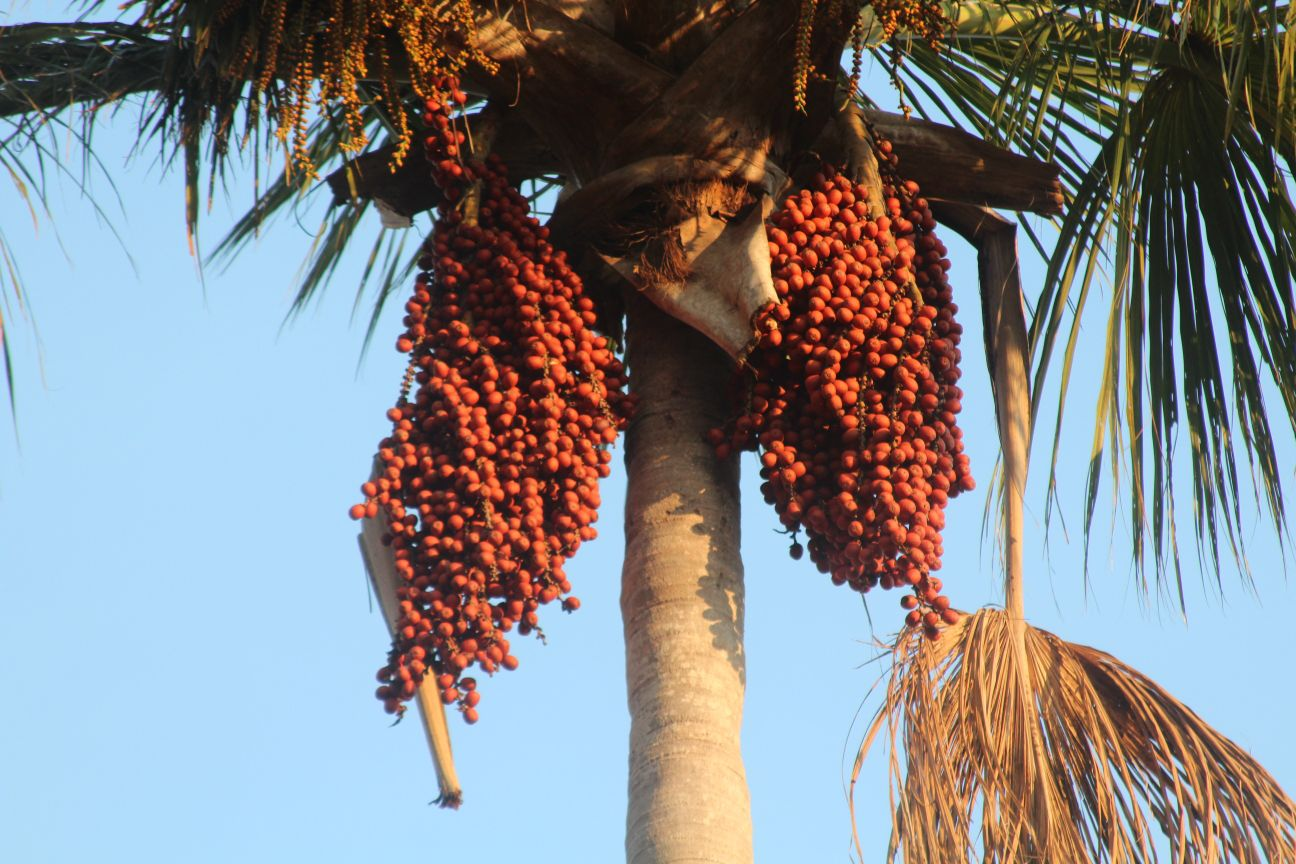
\includegraphics[scale=0.15]{Buriti}
   \caption{Imagem reduzia a $15\%$ do seu tamanho}
\end{figure}
\end{lstlisting}
\end{tcolorbox}
\begin{figure}[H]
   \centering
   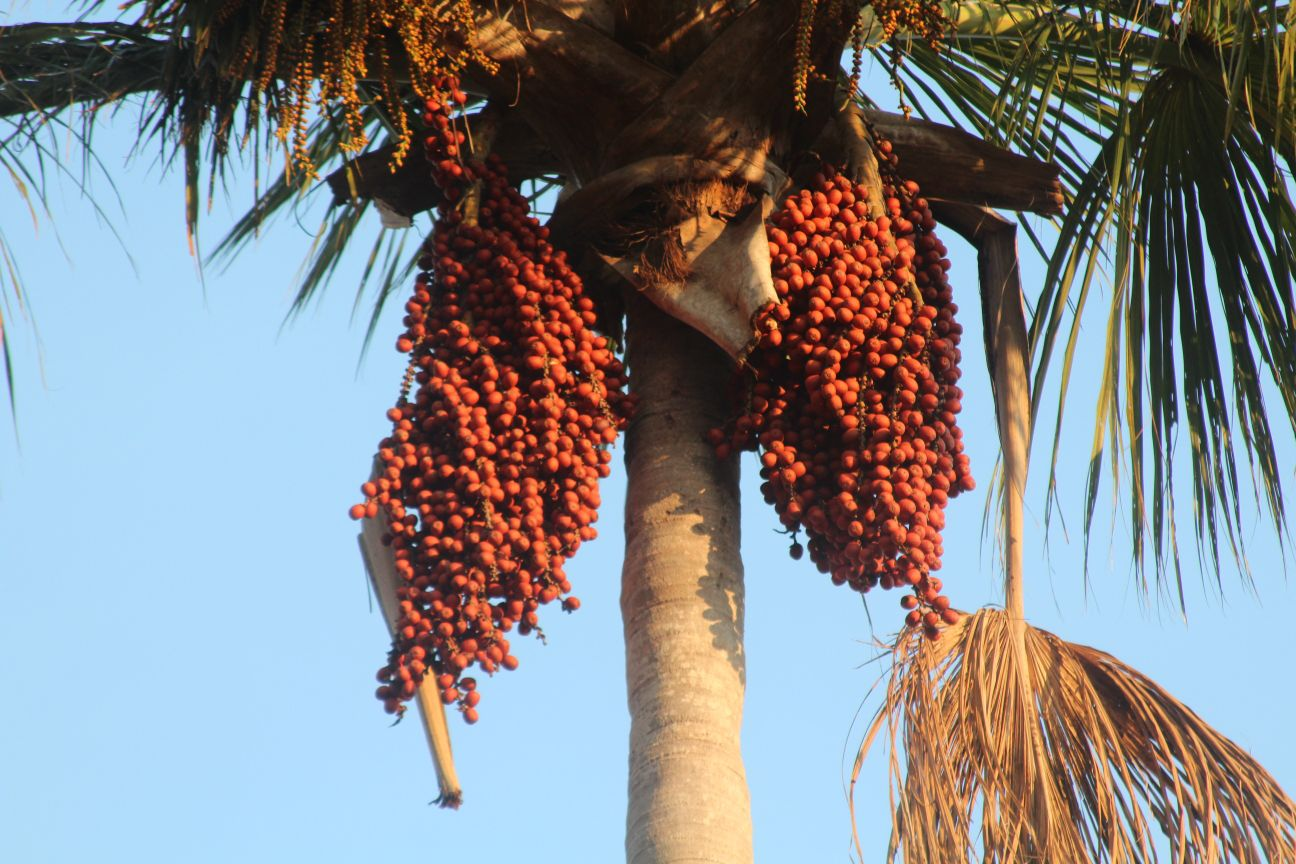
\includegraphics[scale=0.15]{Buriti}
   \caption{Imagem reduzia a $15\%$ do seu tamanho}
   \label{primeira}
\end{figure}

Uma opção muito comum ao lidar com imagem consiste em ajustar seu tamanho para coincidir com a largura da página, o comando \verb|\resizebox| faz esse ajuste
\begin{tcolorbox}
\begin{lstlisting}
\begin{figure}[H]
   \resizebox{\textwidth}{!}{
\includegraphics{RuralP1}}
   \caption{O prédio principal da UFRRJ, vulgo P1}
   \label{op1} %%% Marca para referência cruzada
\end{figure}
\end{lstlisting}
\end{tcolorbox}
\begin{figure}[H]
	\resizebox{\textwidth}{!}{
\includegraphics{RuralP1}}
	\caption{O prédio principal da UFRRJ, vulgo P1}
	\label{op1}
\end{figure}

\subsection{Girando de imagem}

É muito simples girar uma imagem no sentido horário ou anti-horário.
\begin{tcolorbox}
\begin{lstlisting}
\begin{figure}[H]
   \centering
   
\includegraphics[scale=0.1,angle=-15]{Buritis}
   
\includegraphics[scale=0.1]{Buritis}
   
\includegraphics[scale=0.1,angle=15]{Buritis}
   \caption{Girando imagens}\label{giraas}
\end{figure}
\end{lstlisting}
\end{tcolorbox}

\begin{figure}[H]
	\centering
	
\includegraphics[scale=0.1,angle=-15]{Buritis}
	
\includegraphics[scale=0.1]{Buritis}
	
\includegraphics[scale=0.1,angle=15]{Buritis}
	\caption{Girando imagens}\label{giraas}
\end{figure}


\subsection{Imagens lado a lado}

\begin{tcolorbox}
\begin{lstlisting}
\begin{figure}[H]
   \centering
   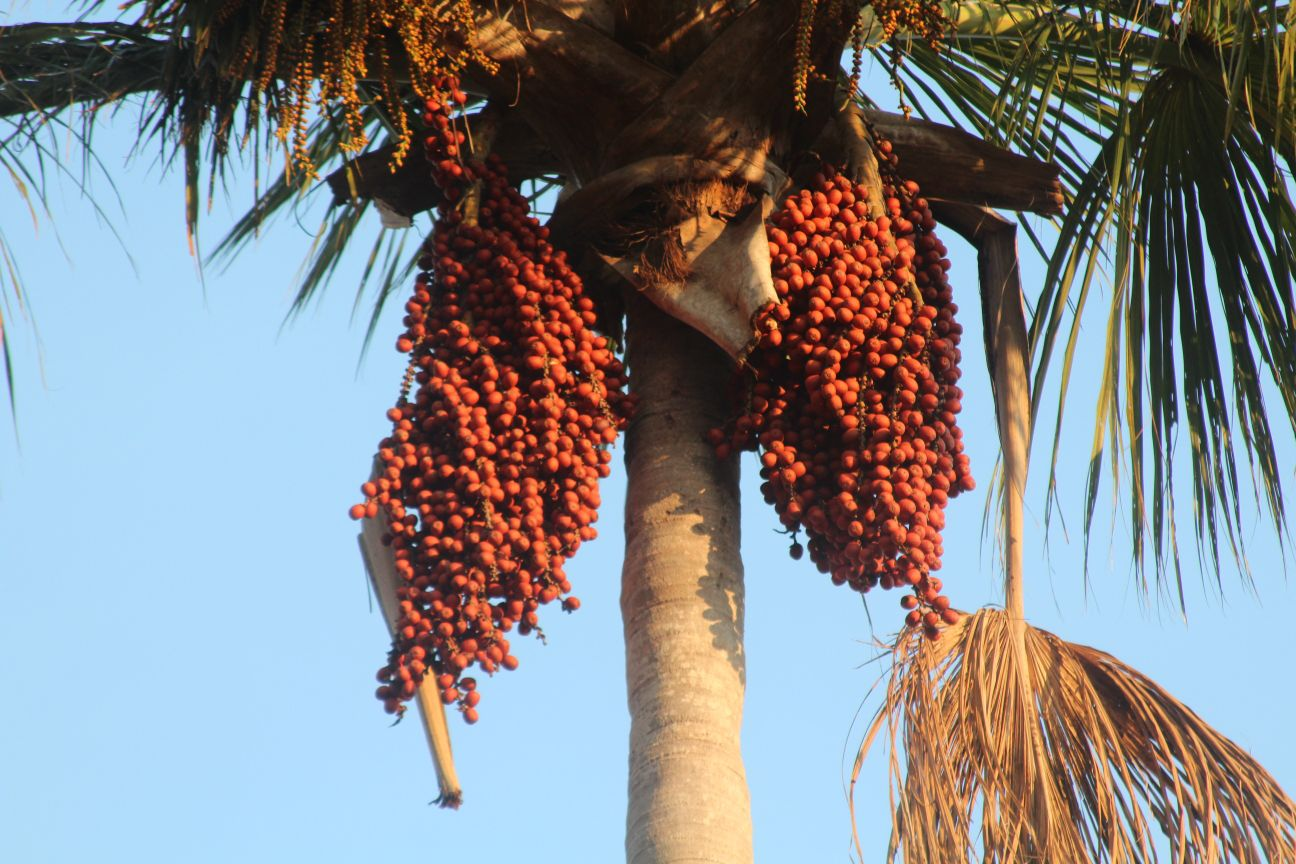
\includegraphics[scale=0.1]{Buriti}
   
\includegraphics[scale=0.1]{RuralP1}
   
\includegraphics[scale=0.1]{Pordosol}
   \caption{Imagens lado a lado}\label{ladoalado}
\end{figure}
\end{lstlisting}
\end{tcolorbox}

\begin{figure}[H]
	\centering
	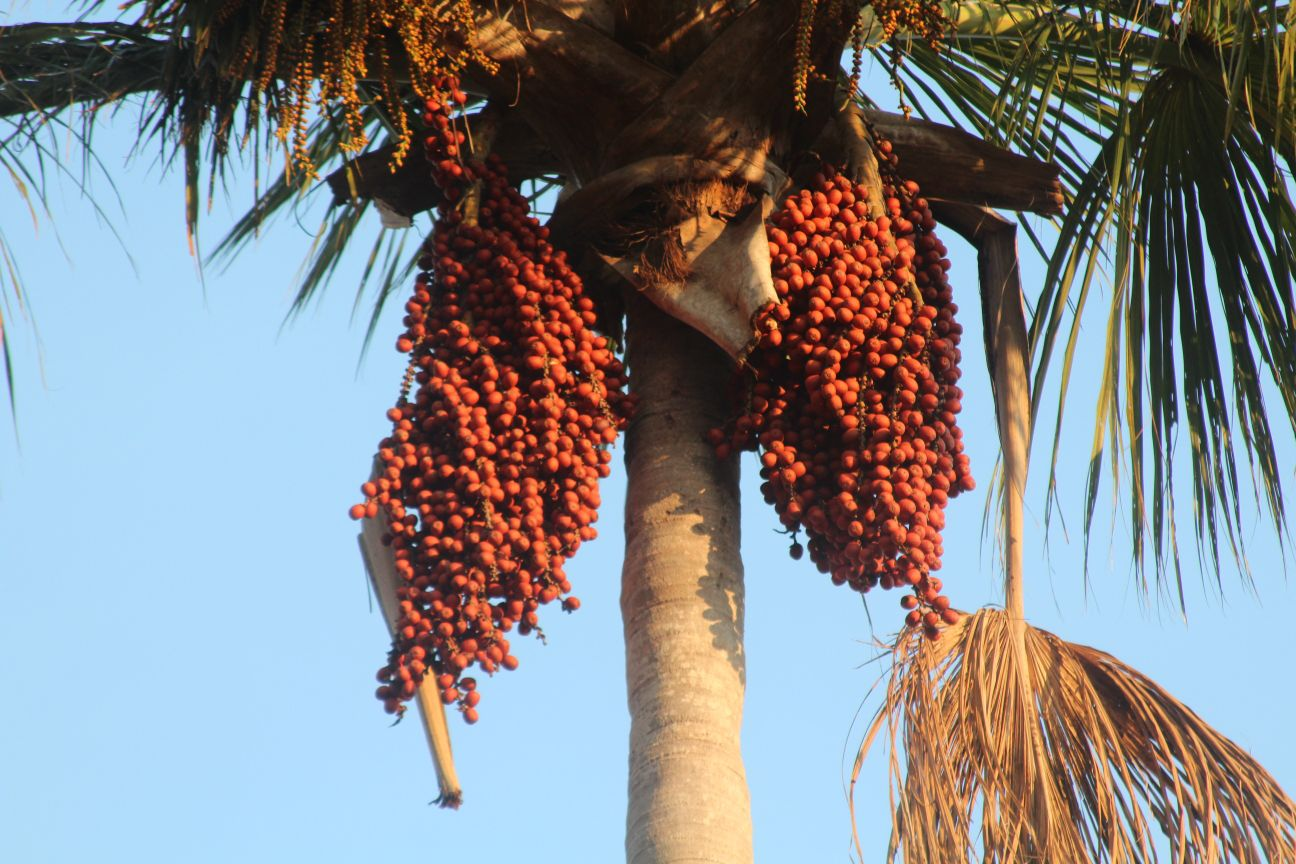
\includegraphics[scale=0.1]{Buriti}
	
\includegraphics[scale=0.1]{RuralP1}
	
\includegraphics[scale=0.1]{Pordosol}
	\caption{Imagens lado a lado}\label{ladoalado}
\end{figure}

Para inserir uma legenda para cada figura e uma legenda geral tem-se a seguinte opção
\begin{tcolorbox}
\begin{lstlisting}
\begin{figure}[H]
   \centering
   \subcaptionbox{Fruta do buriti \label{fruta}}[0.33\linewidth]{%
		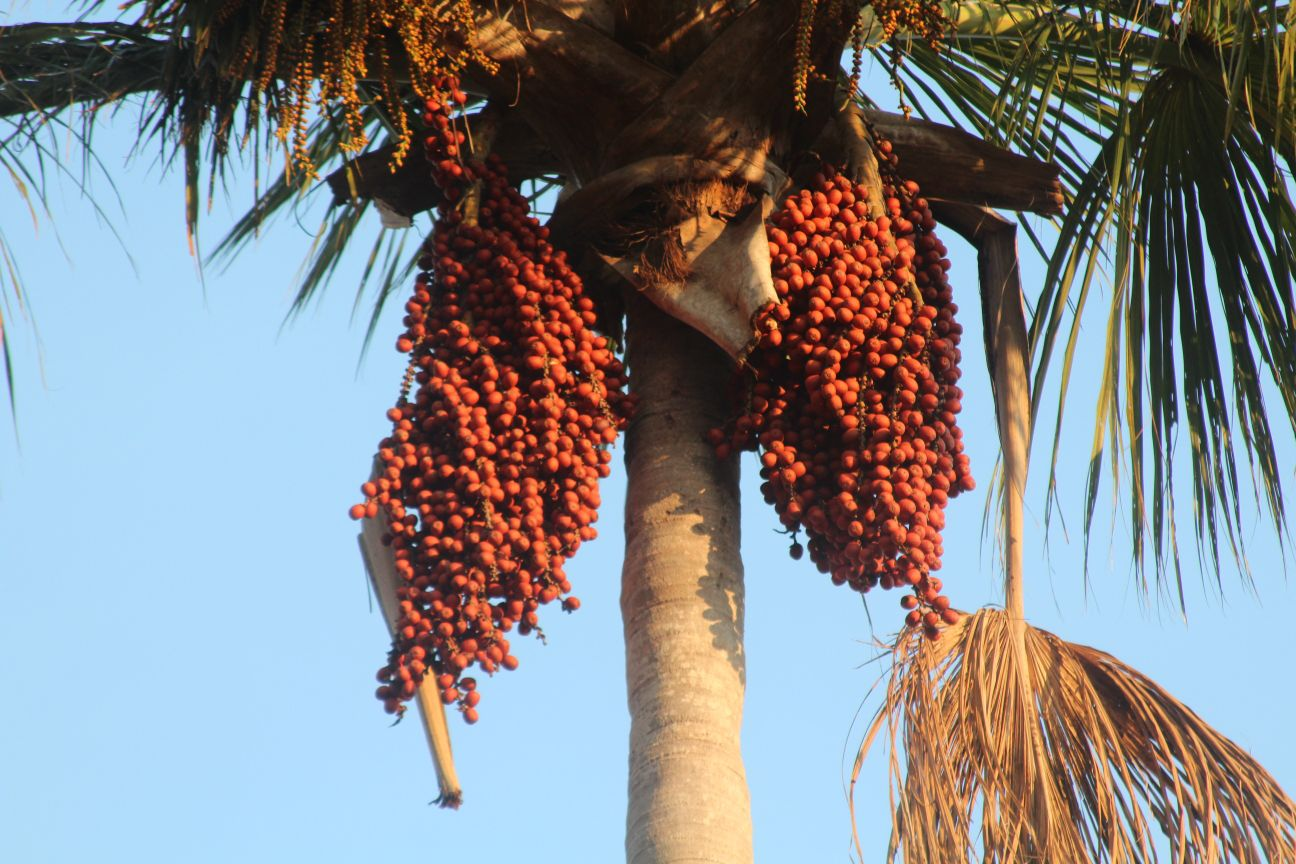
\includegraphics[scale=0.1]{Buriti}} %
   \subcaptionbox{Bonito por do sol e uma sublegenda intencionalmente
        grande\label{Pordosol}}[0.33\linewidth]{%%%
        
\includegraphics[scale=0.1]{Pordosol}}
   \subcaptionbox {Duas palmeiras de buriti \label{duas}}[%%%
        0.3\linewidth]{
\includegraphics[scale=0.12]{Buritis}} %
   \caption{Buriti é uma palmeira de fruto saboroso}\label{buritis}
\end{figure}
\end{lstlisting}
\end{tcolorbox}
\begin{figure}[H]
	\centering
	\subcaptionbox{Fruta do buriti \label{fruta}}[0.33\linewidth]{%
		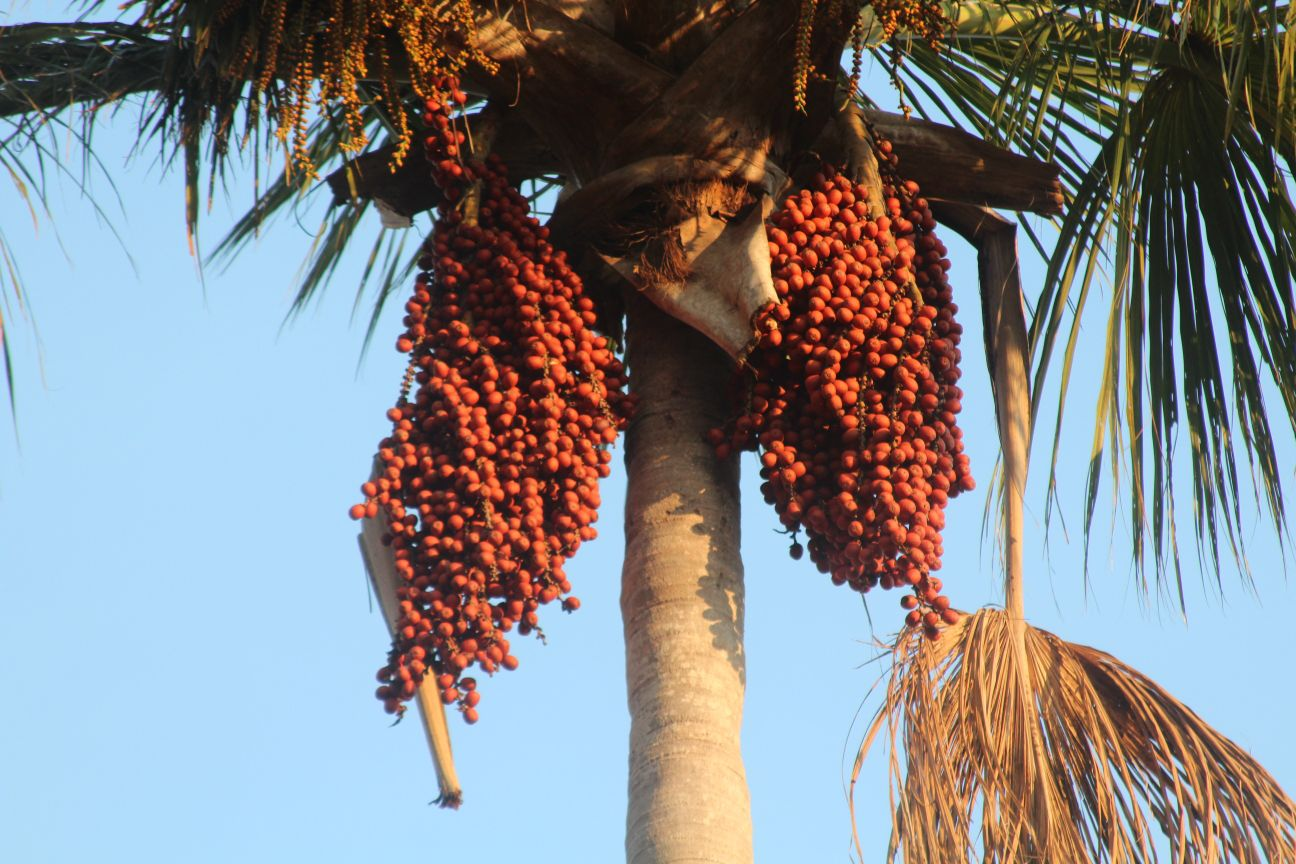
\includegraphics[scale=0.1]{Buriti}} %
	\subcaptionbox{Bonito por do sol e uma sublegenda intencionalmente grande
		\label{Pordosol}}[0.33\linewidth]{
\includegraphics[scale=0.1]{Pordosol}}
	\subcaptionbox {Duas palmeiras de buriti \label{duas}}[0.3\linewidth]{%%%
		
\includegraphics[scale=0.12]{Buritis}} %
	\caption{Buriti é uma palmeira de fruto saboroso}\label{buritis}
\end{figure}


\section{Inclusão de imagem com a classe estilo}

O comando para inserir imagem é o \verb|\includegraphics{imagem}|. 
Alternativamente a classe estilo definiu os comandos: \verb|\imagem| e 
\verb|\imagemlp|. Esses comandos são muito parecidos, o primeiro insere a imagem 
em tamanho natural, o segundo ajusta a largura da imagem à largura da página sem 
provocar distorções, ambos possuem três argumentos, um opcional e dois 
obrigatórios. Veja o manual.


Tanto o \verb|\imagem| quanto o \verb|\imagemlp| inserem a imagem dentro de um ambiente \texttt{table} carregado com o posicionador H, isso implica que a imagem ficará onde foi inserida de qualquer jeito.

Além de seu nome ser mais simples e fácil de manipular, esses dois comandos se encarregam de inserir todos os bons adereços que uma imagem em geral requer, tornando significativamente mais simples a manipulação de imagem.

A imagem~\ref{primeira} foi inserida com o código
\begin{tcolorbox}
\begin{lstlisting}
\begin{figure}[H]
   \centering
   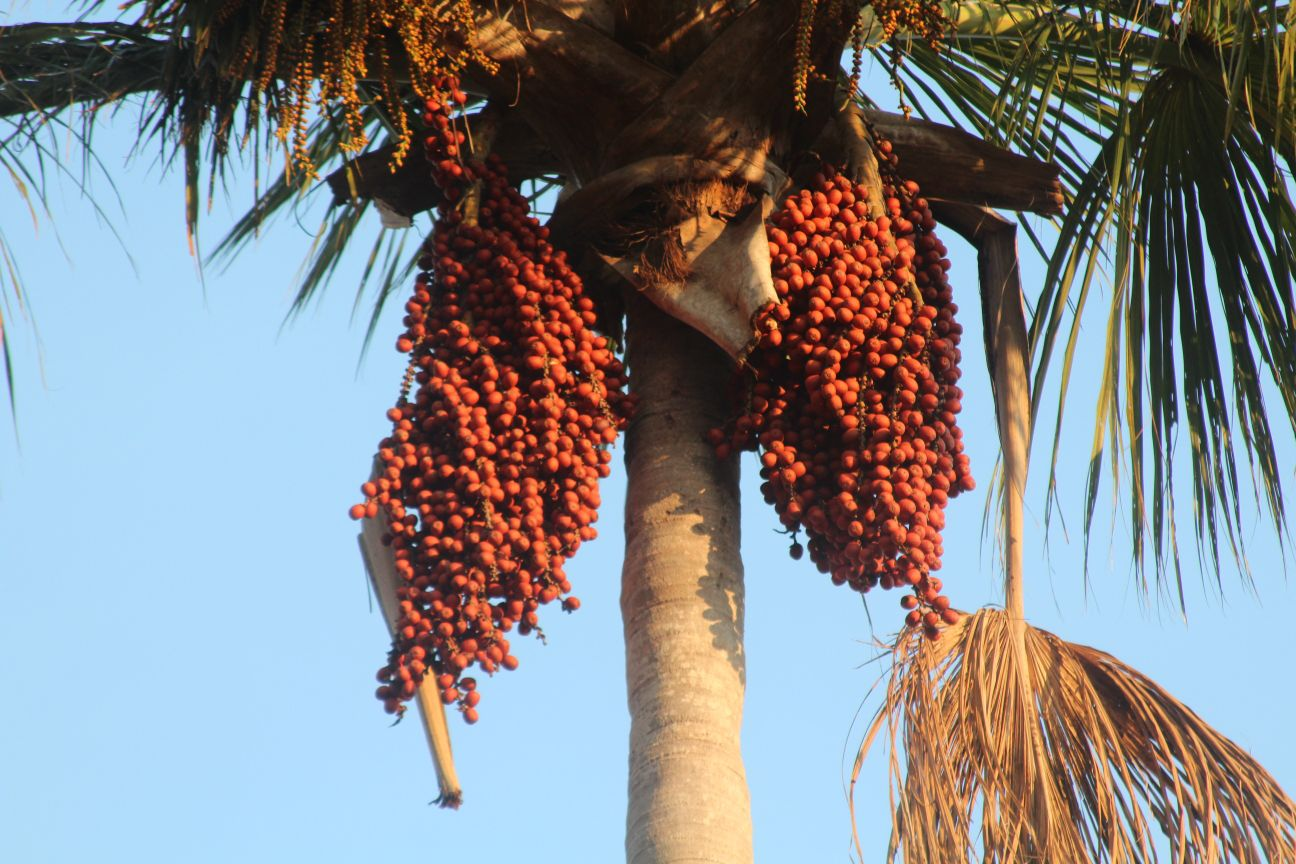
\includegraphics[scale=0.15]{Buriti}
   \caption{Imagem reduzia a $15\%$ do seu tamanho}
\end{figure}
\end{lstlisting}
\end{tcolorbox}

O mesmo resultado é obtido com o singelo fragmento
\begin{tcolorbox}
\begin{lstlisting}
\imagem[scale=0.15]{Buriti}{Imagem reduzia a $15\%$ do seu tamanho}
\end{lstlisting}
\end{tcolorbox}
\imagem[scale=0.15]{Buriti}{Imagem reduzia a $15\%$ do seu tamanho}

Da mesma forma, a imagem~\ref{op1} foi inserida com o código
\begin{tcolorbox}
\begin{lstlisting}
\begin{figure}[H]
   \resizebox{\textwidth}{!}{
\includegraphics{RuralP1}}
   \caption{O prédio principal da UFRRJ, vulgo P1}
   \label{op1} %%% Marca para referência cruzada
\end{figure}
\end{lstlisting}
\end{tcolorbox}

O mesmo resultado é obtido com o código
\begin{tcolorbox}
\begin{lstlisting}
\imagemlp{RuralP1}{O prédio principal da UFRRJ, vulgo P1}
\end{lstlisting}
\end{tcolorbox}
\imagemlp{RuralP1}{O prédio principal da UFRRJ, vulgo P1}


\begin{tcolorbox}
\begin{lstlisting}
   Note que a imagem~\ref{RuralP1} foi ajustada para a largura da página, enquanto a imagem~\ref{Buriti}, por meio do argumento opcional $scale=0.15$, teve seu tamanho reduzido a $15\%$.
\end{lstlisting}
\tcblower
Note que a imagem~\ref{RuralP1} foi ajustada para a largura da página, enquanto a imagem~\ref{Buriti}, por meio do argumento opcional $scale=0.15$, teve seu tamanho reduzido a $15\%$.
\end{tcolorbox}

Observe como a referência cruzada foi feita utilizando o próprio nome do arquivo da imagem, sem necessidade de incluir o \verb|\label{RuralP1}| e \verb|\label{Buriti}|, essa é uma vantagem de usar os comandos da classe estilo.

\imagem{Esquema}{Imagem em pdf}
\chapter{Códigos}\label{codigos}

Há duas formas para inserir um código, ambas exigem que seja carregada a 
opção de classe ``codigo''. Carregada essa opção ficam disponíveis as 
ferramentas do pacote \texttt{listings}, as duas principais são exemplificadas 
a seguir.

\section{Inserindo o código de um arquivo}

Essa possibilidade não admite os acentos ortográficos da língua portuguesa, 
mesmo que estejam em comentário. Mas se o código for copiado para o arquivo tex
os acentos não serão um problema.

Para que o \LaTeX\ dê o devido tratamento ao conteúdo do arquivo 
deve-se informar a qual linguagem o código pertence. São aceitas 
muitas linguagens e alguns dialetos de linguagens, para ver a 
lista completa veja o manual do pacote \pacote{listings}.
Algumas exemplos:

Para inserir código do Matlab use \epar{language}{Matlab}

Para inserir código do Maple use \epar{language}{Maple}.

Para inserir código do C use \epar{language}{C}.

Para inserir código do C++ use \epar{language}{C++}.

Para inserir código do Java use \epar{language}{Java}.

Para inserir código do Fortran use \epar{language}{Fortran}.

Para inserir código do Python use \epar{language}{Python}.

Para inserir código do Pascal use \epar{language}{Pascal}.

Para inserir código do Octave use \epar{language}{Octave}.

No exemplo a seguir foi utilizado um código do matlab, por isso
foi inserida a chave \epar{language}{Matlab} para dizer ao \LaTeX\
que o conteúdo do arquivo Laplace.m é um código do MatLab.

\begin{tcolorbox}[breakable]
\begin{lstlisting}
   \lstinputlisting[language=Matlab,captionpos=b]{Laplace.m}
\end{lstlisting}
\tcblower
\lstinputlisting[language=Matlab,captionpos=b]{Laplace.m}
\end{tcolorbox}

\section{Inserindo o código diretamente}

Para inserir um código basta colocá-lo dentro do ambiente \textsf{lstlisting}. Sua sintaxe é:
\begin{center}
	\begin{minipage}{0.7\textwidth}
		\azul{\coma{begin}}$\{$\verde{\textsf{lstlisting}}$\}$[\op{opções}]
		
		\vspace{0.2cm}
		\hspace{0.5cm}\textit{Conteúdo do ambiente, o código.}
		\vspace{0.2cm}
		
		\azul{\coma{end}}$\{$\textsf{\verde{lstlisting}}$\}$
	\end{minipage}
\end{center}

\begin{tcolorbox}[breakable,title={Código posto dentro de um ambiente lstlisting}]
\begin{lstlisting}[language=Matlab,
caption={Exemplo de inclusão de código},captionpos=b]
m = input('Digite o numero de linhas ');
n = input('Digite o numero de colunas ');
%%% Montando a Matriz do sistema Bloco diagonal
A = zeros(n,m);
nl1 = n - 1;  np1 = n + 1;
msize = n*m;  msln = msize - n;
%%% As três diagonais: Diagonal principal, acima e abaixo
A(1,1) = -4.0; %%% Primeiro valor da diagonal principal
for i = 2:msize
   A(i-1,i) = 1.0;  %%% Abaixo
   A(i,i)   =-4.0;  %%% Valores da diagonal principal
   A(i,i-1) = 1.0;  %%% Acima
end
% Correção: Substituindo alguns valores 1 por 0
for i = n:n:msln
   A(i,i+1) = 0.0;
   A(i+1,i) = 0.0;
end
%%% Diagonais afastadas
for i = np1:msize
   A(i,i-n) = 1.0;
   A(i-n,i) = 1.0;
end
%%% Lado direito do sistema (inclui os valores de fronteira)
b=zeros(msize,1);
%%% Atualiza os valores não nulos
for i = n:n:msize
   b(i,1) = -100;
end
u = A\b % Solução do sistema linear.
% Ordenamento matricial dos valores da temperatura
k = 0;
for i = 1:m
   for j = 1:n
      k = k + 1;
      Temp(i,j) = u(k);
   end
end
Temp
\end{lstlisting}

\end{tcolorbox}






\addcontentsline{toc}{chapter}{Referências}  %%% Só é necessário quando 
%%% a opção glenn é carregada, que é o caso.
\renewcommand{\bibname}{Referências} %%% Para contornar o babel.
\bibliographystyle{unsrtnat}
\bibliography{bibliografia}   %%% Insere o arquivo bibliografia.bib que deve
%%% ficar na mesma paste de seu arquivo tex.
\end{document}

